\section{Intent Resolution}

Given our definitions, we may now attack the problem of intent resolution for our CAIS.
Ideally, any action carried out by our humans within the room would be as explicit
as possible. Indeed, when using something like MUIFOLD, this explicitness is handled for
the user under the hood by the app, tying together what note or block they're interacting
with, and what action they're attempting to accomplish with it. However, through voice,
providing the full explicit action may be difficult or impossible. To demonstrate this
behavior in more exact terms, we provide an example. Imagine that within a CAIS, there
are two agents working with the sticky notes domain. One of the notes that has been
created is a green note. After a period of time, one of the agents wants to delete that
green note, and so utters the sentence ``Delete the green note'' to the CAIS. From our
conversation-worker for this sentence, we receive the ``$\delete$'' intent and a ``green''
entity. Within the orchestrator, our intent is matched with the following candidate action:

\begin{lstlisting}[caption=delete action for the note,label={lst:strips}]
    (define-action delete1 [?x] {
            :preconditions [(onScreen ?x)]
            :additions     []
            :deletions     [(onScreen ?x)]
    })
\end{lstlisting}

From this action, we are looking for a ``?x'' that is of the \Note sort, and fits our
precondition of it being on the screen. Additionally, we know from the derived entity of
our sentence that the note is also green. We combine this information into the query
``$\exists(\Note\ x)((onScreen\ x) \land (isColor\ x\ green))$'', or in plain english, does there exist 
a note such that the note is on the screen and is green. We then run this query through
ShadowProver with the query as our goal statement and the CAIS' knowledge about the current
state of affairs from our knowledge base as our axiom set. From ShadowProver, we derive
a candidate set of notes that fit our criteria. We take this candidate set of notes and
then run from newest to oldest axioms within the knowledge base for the agent who uttered
our sentence, looking for the most recent instance of an axiom that contains one of the
notes from our candidate set, considering both how long ago that axiom is and how many
candidates there are to consider. In this process, we ensure we only consider notes that
have entered our agent's knowledge base via perception or other mechanisms. If there is
then only one note that matches from this process, we then use that note for our action.
If there are more than one note, we then enter into a process of resolution via a small
conditional plan fragment, asking the user for clarification, utilizing a set-up inspired
by work from Botea et al.~\cite{botea_generating_2019} to generate the requisite dialog
nodes via a simplified conditional planner. For example, given we have two possible note
candidates, our system generates the dialogue tree shown in 
Figure~\ref{fig:intent_resolution_fragment}. In this, the CAIS asks the user to pick between
two  notes that they might have meant from their statement. The user is then expected to either
cancel out of the original intent altogether, or by giving the system a specific note number
to use.

\begin{figure}
\centering
  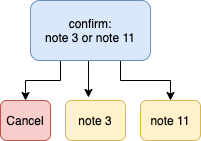
\includegraphics[width=0.4\columnwidth]{chapters/06_planning/figures/intent_resolution_fragment.png}
  \caption{Conditional plan fragment to ask clarification from user.}
  \label{fig:intent_resolution_fragment}
\end{figure}